\chapter{Økonomi} \label{Okonomi}
Formålet med dette afsnit er ud fra et økonomisk aspekt, at vurdere - så vidt muligt sort på hvidt - om en given teknologisk løsning er værd at implementere i praksis. I dette tilfælde, gøres det ved at bruge omkostningsminimeringsanalysen. Da det antages at den sundhedsmæssige effekt er ens i den nuværende situation og i den fremtidige situation, hvor robotarmen implementeres som en add-on løsning til eksisterende ultralydsudstyr. \\
Der opstilles to scenarier. I begge scenarier sammenlignes nuværende udgifter til ultralydsudstyr med udgifterne til implementering af ultralyds robotarm, hvorefter der udarbejdes en økonomisk vurdering af hvert scenarie. I første scenarie er det ”Afdelingen for Kvindesygdomme og fødsler” på Skejby Hospital og i andet scenarie er det ”Kvindeafdelingen, Svangre- og ultralydsambulatorium” på Hospitalsenheden Horsens. 

Vurderingen tager udgangspunkt i det senest indkøbte ultralydsudstyr på de pågældende afdelinger. Indkøbspriserne på udstyret er estimeret. Da robotarmen ikke er færdigudviklet, er det vigtigt at pointere at indkøbsprisen på 400.000 kr. for robotarmen med tilhørende nødvendig udstyr er baseret på hvad CEO hos Robotic Ultrasound, Søren Pallesen forventer, at salgsprisen på robotarmen bliver, når den kommer på markedet. Alle priser i de følgende beregninger er angivet uden moms. 

\section{Scenarie 1}
I dette scenarie er det valgt at tage udgangspunkt i det udstyr der benyttes ved en nakkefoldsscanning i 11. til 13. uge uden komplikationer på ”Afdelingen for Kvindesygdomme og fødsler” på Skejby Hospital. Dette udstyr består af C1-5-RS convex transducer, software til avancerede 3D/4D billeder samt printer med tilbehør, den samlede pris på dette er 223.000 kr. (reference). 

Ifølge Tina Arnbjørn, afdelingssygeplejerske på ”Kvindeafdelingen” på Hospitalsenheden Horsens skal IT-udstyr afskrives over 10 år, da udstyret er forældet efter denne periode. Derfor fordeles etableringsomkostningerne over ti år efter annuitetsmetoden med forrentningsfaktor på 2,1 \%. Forrentningsfaktoren er estimeres til at være et gennemsnit af inflations renten i Danmark i 2016 og 2020 (reference). \\
Samlet løber etableringsomkostninger til det eksisterende udstyr på Skejby op i 223.000 kr. (se bilag 1). Fordelt ligeligt ud på ti år bliver dette med en forrentningsfaktor på 2,1 \% til 25.086 kr. årligt.
\begin{figure}[H]\centering
	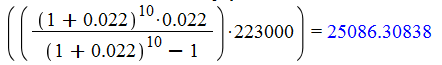
\includegraphics[width = 0.7\textwidth]{Figurer/SkejbyOkonomi}
	\caption{Annuitetsberegning for ultralydsudstyr, Skejby Hospital}
	\label{SkejbyOkonomi}
\end{figure}
Ses der på den fremtidige situation, hvor udgifterne til robotarmen medtages løber etableringsomkostninger op i 623.000 kr. (se bilag 1). Fordelt ligeligt ud på ti år bliver dette med en forrentningsfaktor på 2,1 \% til 70.084 kr. årligt. 
\begin{figure}[H]\centering
	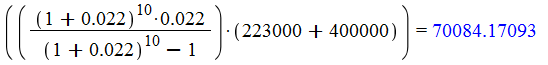
\includegraphics[width = 0.8\textwidth]{Figurer/SkejbyRobotOkonomi}
	\caption{Annuitetsberegning for ultralydsudstyr samt robotarm, Skejby Hospital}
	\label{SkejbyRobotOkonomi}
\end{figure}
Heraf ses det tydeligt at udgifterne til implementering af robotarmen på årlig basis er markant højere end til implementering af nuværende udstyr. 

Afsnit herunder med kursiv er ikke færdig skrevet, her mangler vi specielt dit syn på sagen inden vi går videre… \\
\textit{I det følgende antages det at implementeringen af robotarmen vil kunne spare en sonograf grundet bedre arbejdsforhold, hvilket er nærmere begrundet i organisations-afsnittet. Månedslønnen for en sonograf med 2 års erfaring med kvalifikationstillæg er på løntrin 6, hvilket giver 26.967 kr. På årsbasis giver det en årsløn på 323.604 kr.  (Reference - udover Horsens)}

\section{Scenarie 2}
I dette scenarie tages der udgangspunkt i et fuldt sæt ultralydsudstyr, som kan benyttes ved alle typer af scanninger i løbet af en graviditets periode (reference). Udstyret er placeret på ”Kvindeafdelingen, Svangre- og ultralydsambulatorium” på Hospitalsenheden Horsens, hvor de har fem stuer med ens udstyr. I dette scenarie beregnes der udelukkende på udgifterne til, at holde en stue i drift. \\
Det estimeres at udstyret er forældet efter ti år (reference), og derfor fordeles etableringsomkostningerne over ti år efter annuitetsmetoden med forrentningsfaktor på 2,1 \%. Forrentningsfaktoren er estimeres til at være et gennemsnit inflations renten i Danmark i 2016 og 2020.  \\
Etableringsomkostninger på et fuldt sæt udstyr i den nuværende situation er samlet set på 850.000 kr. (se bilag 1):
\begin{figure}[h!]\centering
	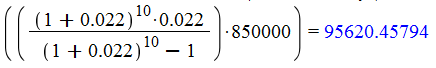
\includegraphics[width = 0.7\textwidth]{Figurer/HorsensOkonomi}
	\caption{Annuitetsberegning for ultralydsudstyr, Hospitalsenheden Horsens}
	\label{HorsensOkonomi}
\end{figure}

Den fremtidige situation beregnes ligeledes efter annuitetsmetoden, hvor det antages at det nuværende udstyr vil blive brugt i sammenkobling med robotarmen, grundet at robotarmen er en add-on løsning. Samlet set er etableringsomkostningerne dermed på 1.250.000 kr.:
\begin{figure}[h!]\centering
	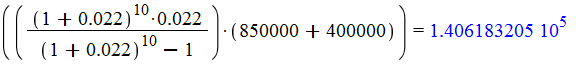
\includegraphics[width = 0.8\textwidth]{Figurer/HorsensRobotOkonomi}
	\caption{Annuitetsberegning for ultralydsudstyr samt robotarm, Hospitalsenheden Horsens}
	\label{HorsensRobotOkonomi}
\end{figure}

\section{Delkonklusion}

